\documentclass[11pt]{article}
\usepackage{amsmath, amssymb, physics, mathtools, bm}
\usepackage{tikz, pgfplots}
\usetikzlibrary{decorations.pathmorphing, arrows.meta}
\pgfplotsset{compat=1.18}
\usepackage[margin=2.3cm]{geometry}
\usepackage{siunitx, booktabs, hyperref}
\usepackage{braket}

\newcommand{\de}{\mathrm{d}}
\newcommand{\Lap}{\nabla^{2}}

\title{B3: Atomic and Laser Physics --- MT 2020 Model Solutions}
\author{}
\date{}

\begin{document}
\maketitle

%==========================================================================
\section*{Question 1 --- Central field, Thomas--Fermi atom}
%==========================================================================

\textbf{Problem.} For an $N$-electron atom: (a) state the central-field approximation and the good quantum numbers; (b) sketch the effective potential of sodium; (c) using a Fermi-gas description ($n=8\pi p^3/3h^3$) derive the Thomas--Fermi equation $\chi''=\chi^{3/2}/x^{1/2}$ with $x=r/b$ and find $b$; (d) discuss its limits; (e) explain why $4s$ fills before $3d$ in K.

\subsection*{(a)}

The two-body term $\sum_{i>j}e^2/(4\pi\varepsilon_0 r_{ij})$ prevents separation. Replace by spherical mean acting on each electron:
\[
\sum_{i>j}\frac{e^2}{4\pi\varepsilon_0 r_{ij}}\;\longrightarrow\;\sum_i S(r_i).
\]
Each electron sees a central potential:
\[
U(r)=-\frac{Ze^2}{4\pi\varepsilon_0 r}+S(r).
\]
Hamiltonian becomes a sum of one-electron terms; orbitals are labelled by single-particle quantum numbers:
\[
\boxed{\;n,\;\ell,\;m_\ell,\;m_s\;}
\]
Energies depend on $n$ and $\ell$ (non-Coulombic). Residual electron repulsion couples individual $\ell_i,s_i$ so only $L,S,J,M_J$ are strictly good for the full atom.

\subsection*{(b)}

Two limits set the shape of $U(r)$ for Na ($Z=11$, 10 core electrons):
\[
r\to 0:\quad U(r)\to -\frac{Ze^2}{4\pi\varepsilon_0 r}.
\]
\[
r\to\infty:\quad U(r)\to -\frac{e^2}{4\pi\varepsilon_0 r}.
\]
Screening turns on over $r\sim a_0$.

\begin{center}
\begin{tikzpicture}[>=stealth, scale=1.0]
  \draw[->] (0,0) -- (8.0,0) node[right] {$r$};
  \draw[->] (0,-4.4) -- (0,1.2) node[above] {$U(r)$};
  \draw[domain=0.25:0.95, smooth, variable=\x, thick, blue] plot ({\x},{-1.7/\x});
  \draw[domain=1.7:7.5, smooth, variable=\x, thick, red]  plot ({\x},{-0.4/\x});
  \draw[dashed, thick] (0.95,{-1.7/0.95}) .. controls (1.15,-1.2) and (1.4,-0.55) .. (1.7,{-0.4/1.7});
  \node[blue, anchor=west] at (1.2,-3.6) {$-\dfrac{Ze^2}{4\pi\varepsilon_0 r}\;(r\to 0)$};
  \node[red,  anchor=west] at (5.0,-0.35) {$-\dfrac{e^2}{4\pi\varepsilon_0 r}\;(r\to\infty)$};
  \node[anchor=south] at (3.6,0.55) {screening region $r\sim a_0$};
  \draw[->] (3.0,0.5) -- (1.4,-0.45);
  \node[circle, fill, inner sep=1.2pt, label=below right:{core $\sim 10\,e^-$}] at (1.3,-1.3) {};
\end{tikzpicture}
\end{center}

\subsection*{(c)}

Let $V(r)$ be the electric potential of the screened nucleus, positive near origin. Electron PE is $-eV$. Just-bound condition $p_F^2/(2m)-eV=0$:
\[
p_F^2/(2m)=eV(r).
\]
Solve for $p_F$:
\[
p_F(r)=\bigl[2meV(r)\bigr]^{1/2}.
\]
Insert into the given density $n=8\pi p^3/(3h^3)$ with $p=p_F$:
\[
n_e(r)=\frac{8\pi}{3h^3}\bigl[2meV(r)\bigr]^{3/2}.
\]
Parametrise with screening function $\chi$, $Z_\text{eff}=\chi Z$, BCs $\chi(0)=1$, $\chi(\infty)=0$:
\[
V(r)=\frac{Z e\,\chi(r)}{4\pi\varepsilon_0 r}.
\]
Multiply by $e$:
\[
eV(r)=\frac{Ze^2\chi(r)}{4\pi\varepsilon_0 r}.
\]
Substitute into $n_e$:
\[
n_e(r)=\frac{8\pi}{3h^3}\!\left[\frac{2me^2 Z\chi}{4\pi\varepsilon_0 r}\right]^{3/2}.
\]
Poisson's equation with electron charge density $\rho_e=-en_e$:
\[
\Lap V=-\rho_e/\varepsilon_0=\frac{e\,n_e(r)}{\varepsilon_0}.
\]
Use the radial identity:
\[
\Lap V=\frac{1}{r}\frac{\de^2(rV)}{\de r^2}.
\]
Substitute $rV=Ze\chi/(4\pi\varepsilon_0)$:
\[
\frac{Ze}{4\pi\varepsilon_0}\frac{1}{r}\frac{\de^2\chi}{\de r^2}=\frac{e}{\varepsilon_0}\frac{8\pi}{3h^3}\!\left[\frac{2me^2 Z\chi}{4\pi\varepsilon_0 r}\right]^{3/2}.
\]
Multiply both sides by $4\pi\varepsilon_0 r/(Ze)$:
\[
\frac{\de^2\chi}{\de r^2}=\frac{4\pi r}{Z}\cdot\frac{8\pi}{3h^3}\cdot\frac{(2me^2 Z)^{3/2}\chi^{3/2}}{(4\pi\varepsilon_0 r)^{3/2}}.
\]
Cancel one $Z$ against $Z^{3/2}$:
\[
\frac{\de^2\chi}{\de r^2}=\frac{32\pi^2}{3h^3}\cdot\frac{(2m)^{3/2}e^3 Z^{1/2}}{(4\pi\varepsilon_0)^{3/2}}\,\frac{\chi^{3/2}}{r^{1/2}}.
\]
Collect powers of $r$ and constants:
\[
\frac{\de^2\chi}{\de r^2}=C\,\frac{\chi^{3/2}}{r^{1/2}},\qquad
C=\frac{32\pi^2}{3h^3}\,\frac{(2m)^{3/2}e^3 Z^{1/2}}{(4\pi\varepsilon_0)^{3/2}}.
\]
Set $r=bx$, so $\de^2/\de r^2=(1/b^2)\de^2/\de x^2$:
\[
\frac{1}{b^2}\frac{\de^2\chi}{\de x^2}=C\,\frac{\chi^{3/2}}{b^{1/2}x^{1/2}}.
\]
Demand the universal form $\chi''(x)=\chi^{3/2}/x^{1/2}$:
\[
\frac{1}{b^2}=\frac{C}{b^{1/2}}.
\]
Multiply by $b^{1/2}$:
\[
b^{-3/2}=C.
\]
Invert:
\[
b^{3/2}=\frac{1}{C}.
\]
Take the $2/3$ power:
\[
b=C^{-2/3}=\left(\frac{3h^3(4\pi\varepsilon_0)^{3/2}}{32\pi^2(2m)^{3/2}e^3 Z^{1/2}}\right)^{\!2/3}.
\]
Apply the $2/3$ to each factor:
\[
b=\left(\frac{3h^3}{32\pi^2}\right)^{\!2/3}\frac{(4\pi\varepsilon_0)}{(2m)e^2 Z^{1/3}}.
\]
Pull out the $Z$ dependence:
\[
b=\left(\frac{3h^3}{32\pi^2}\right)^{\!2/3}\frac{4\pi\varepsilon_0}{2m e^2}\,Z^{-1/3}.
\]
Substitute $h=2\pi\hbar$, so $h^3=8\pi^3\hbar^3$:
\[
\frac{3h^3}{32\pi^2}=\frac{3\cdot 8\pi^3\hbar^3}{32\pi^2}=\frac{3\pi\hbar^3}{4}.
\]
Raise to $2/3$:
\[
\left(\frac{3h^3}{32\pi^2}\right)^{\!2/3}=\left(\frac{3\pi\hbar^3}{4}\right)^{\!2/3}=\frac{(3\pi)^{2/3}}{4^{2/3}}\hbar^2.
\]
Use the Bohr radius $a_0=4\pi\varepsilon_0\hbar^2/(me^2)$:
\[
\frac{4\pi\varepsilon_0}{2m e^2}=\frac{a_0}{2\hbar^2}.
\]
Combine:
\[
b=\frac{(3\pi)^{2/3}}{4^{2/3}}\hbar^2\cdot\frac{a_0}{2\hbar^2}\,Z^{-1/3}.
\]
Cancel $\hbar^2$:
\[
b=\frac{(3\pi)^{2/3}}{2\cdot 4^{2/3}}\,a_0 Z^{-1/3}.
\]
Reduce $2\cdot 4^{2/3}=2^{1+4/3}=2^{7/3}=(2^7)^{1/3}=128^{1/3}$:
\[
b=\frac{(3\pi)^{2/3}}{128^{1/3}}\,a_0 Z^{-1/3}.
\]
Combine cube roots using $(3\pi)^{2/3}=(9\pi^2)^{1/3}$:
\[
\boxed{\;b=\left(\frac{9\pi^2}{128\,Z}\right)^{1/3}a_0\approx 0.885\,Z^{-1/3}a_0.\;}
\]

\subsection*{(d)}

Continuum Fermi-gas requires local Fermi wavelength $\ll$ scale on which $V$ varies. Fails near the nucleus ($V\to+\infty$, density diverges), in the outer fringe (few electrons, statistics breaks), and for light atoms (low $N$). Reliable for the core of heavy atoms.

\subsection*{(e)}

In a screened (non-Coulombic) central field, low-$\ell$ orbitals \emph{penetrate} the core and feel a larger $Z_\text{eff}$. Centrifugal barrier $\ell(\ell+1)\hbar^2/(2mr^2)$ excludes $3d$ ($\ell=2$) from the core, so $3d$ sees $Z_\text{eff}\approx 1$. The $4s$ orbital, although higher $n$, has substantial inner radial probability and sits at lower energy than $3d$. Therefore K is $[\text{Ar}]\,4s^1$.

%==========================================================================
\section*{Question 2 --- Hyperfine structure in magnetic fields}
%==========================================================================

\textbf{Problem.} Hamiltonian $\mathcal H=A\vec I\!\cdot\!\vec J+g_J\mu_B\vec J\!\cdot\!\vec B-g_I\mu_N\vec I\!\cdot\!\vec B$. (a) interpret each term; (b) estimate weak-field threshold; (c) derive $\Delta E=\tfrac12 AK+g_F\mu_B B M_F$; (d) draw level diagram for $J=3/2,I=3$; (e) strong-field hydrogen $1s\,{}^2S_{1/2}$, verify ratio.

\subsection*{(a)}

\begin{description}
\item[$A\,\vec I\cdot\vec J$:] magnetic hyperfine coupling between nuclear moment $\propto\vec I$ and the electronic field at the nucleus.
\item[$g_J\mu_B\,\vec J\cdot\vec B$:] electronic Zeeman coupling of $-g_J\mu_B\vec J/\hbar$ to $\vec B$.
\item[$-g_I\mu_N\,\vec I\cdot\vec B$:] nuclear Zeeman coupling; smaller than the electronic term by $\mu_N/\mu_B\sim m_e/m_p\approx 1/1836$.
\end{description}

\subsection*{(b)}

Weak field requires hyperfine $\gg$ electronic Zeeman:
\[
A I\gg g_J\mu_B B.
\]
Solve for the crossover field:
\[
B\ll B^*\equiv\frac{A I}{g_J\mu_B}.
\]
Take alkali ground-state $A/h\sim\SI{1}{GHz}$:
\[
A\sim h\cdot 10^9\,\text{Hz}.
\]
Multiply $h=\SI{6.626e-34}{J.s}$:
\[
A\approx\SI{6.6e-25}{J}.
\]
Plug $g_J\approx 2$, $I\sim 3/2$, $\mu_B=\SI{9.27e-24}{J/T}$:
\[
B^*\sim\frac{(6.6\times 10^{-25})(1.5)}{(2)(9.27\times 10^{-24})}\,\text{T}.
\]
Reduce numerator:
\[
(6.6\times 10^{-25})(1.5)=9.9\times 10^{-25}\,\text{J}.
\]
Reduce denominator:
\[
(2)(9.27\times 10^{-24})=1.85\times 10^{-23}\,\text{J/T}.
\]
Divide:
\[
B^*\approx\SI{0.05}{T}.
\]
\[
\boxed{\;B\lesssim\SI{50}{mT}\;\text{for weak-field regime.}\;}
\]

\subsection*{(c)}

Form $\vec F=\vec I+\vec J$, $F\in\{|I-J|,\dots,I+J\}$. Square the sum:
\[
\vec F^2=\vec I^2+\vec J^2+2\vec I\!\cdot\!\vec J.
\]
Rearrange for the dot product:
\[
\vec I\cdot\vec J=\tfrac12\bigl[\vec F^2-\vec I^2-\vec J^2\bigr].
\]
Take eigenvalues in $\ket{F,M_F}$:
\[
\vec I\cdot\vec J=\tfrac12[F(F+1)-I(I+1)-J(J+1)]\hbar^2.
\]
Absorb $\hbar^2$ into $A$:
\[
\langle A\vec I\cdot\vec J\rangle=\tfrac12 A K,\qquad
\boxed{\;K=F(F+1)-I(I+1)-J(J+1).\;}
\]
Treat Zeeman as perturbation in $\ket{F,M_F}$. Project via Land\'e:
\[
\langle\vec J\rangle=\frac{\vec F\!\cdot\!\vec J}{F(F+1)\hbar^2}\vec F,\qquad
\langle\vec I\rangle=\frac{\vec F\!\cdot\!\vec I}{F(F+1)\hbar^2}\vec F.
\]
Write $\vec J=\vec F-\vec I$ and square:
\[
\vec J^2=\vec F^2+\vec I^2-2\vec F\!\cdot\!\vec J.
\]
Solve for $\vec F\!\cdot\!\vec J$:
\[
\vec F\!\cdot\!\vec J=\tfrac12[F(F+1)+J(J+1)-I(I+1)]\hbar^2.
\]
Write $\vec I=\vec F-\vec J$ and square:
\[
\vec I^2=\vec F^2+\vec J^2-2\vec F\!\cdot\!\vec I.
\]
Solve for $\vec F\!\cdot\!\vec I$:
\[
\vec F\!\cdot\!\vec I=\tfrac12[F(F+1)+I(I+1)-J(J+1)]\hbar^2.
\]
Take $\vec B=B\hat z$ so $\langle F_z\rangle=M_F\hbar$:
\[
\Delta E_\text{Z}=g_J\mu_B B\langle J_z\rangle-g_I\mu_N B\langle I_z\rangle.
\]
Insert projected components:
\[
\Delta E_\text{Z}=\left[g_J\mu_B\,\frac{\vec F\!\cdot\!\vec J}{F(F+1)\hbar^2}-g_I\mu_N\,\frac{\vec F\!\cdot\!\vec I}{F(F+1)\hbar^2}\right]B M_F\hbar.
\]
Drop the nuclear piece ($\mu_N/\mu_B\sim m_e/m_p\ll 1$):
\[
\Delta E_\text{Z}\approx g_J\mu_B B M_F\hbar\,\frac{\vec F\!\cdot\!\vec J}{F(F+1)\hbar^2}.
\]
Substitute $\vec F\!\cdot\!\vec J$:
\[
\Delta E_\text{Z}=g_J\,\frac{F(F+1)+J(J+1)-I(I+1)}{2F(F+1)}\,\mu_B B M_F.
\]
Read off $g_F$:
\[
\boxed{\;g_F=g_J\,\frac{F(F+1)+J(J+1)-I(I+1)}{2F(F+1)},\quad\Delta E=\tfrac12 AK+g_F\mu_B B M_F.\;}
\]

\subsection*{(d)}

For $J=3/2,I=3$, allowed $F\in\{|I-J|,\dots,I+J\}$:
\[
F\in\{3/2,\;5/2,\;7/2,\;9/2\}.
\]
Compute $I(I+1)$ and $J(J+1)$:
\[
I(I+1)=12,\qquad J(J+1)=15/4.
\]
Form $K=F(F+1)-I(I+1)-J(J+1)$:
\[
K=F(F+1)-12-15/4.
\]
Tabulate for each $F$:
\begin{center}
\begin{tabular}{@{}cccc@{}}\toprule
$F$ & $F(F+1)$ & $K$ & $\tfrac12 AK$ \\ \midrule
$3/2$ & $15/4$ & $-12$ & $-6A$ \\
$5/2$ & $35/4$ & $-7$  & $-7A/2$ \\
$7/2$ & $63/4$ & $0$   & $0$ \\
$9/2$ & $99/4$ & $+9$  & $+9A/2$ \\
\bottomrule
\end{tabular}
\end{center}
Each $F$ splits into $2F+1$ Zeeman sublevels: $4+6+8+10=28=(2J+1)(2I+1)$. Sublevel spacing $g_F\mu_B B$ depends on $F$.

\begin{center}
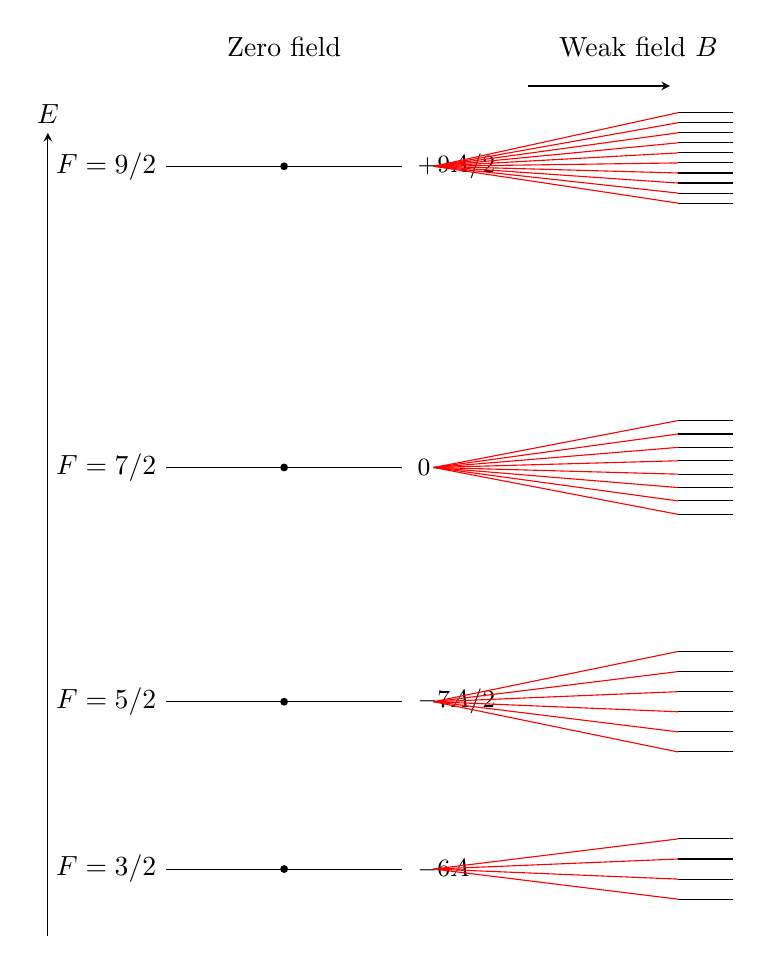
\begin{tikzpicture}[>=stealth, xscale=1.0, yscale=0.85]
  % zero-field levels (left) with markers
  \draw (0,-6) -- (3,-6); \node[circle,fill,inner sep=1pt] at (1.5,-6) {};
    \node[left] at (0,-6) {$F=3/2$}; \node[right=2pt] at (3,-6) {\small $-6A$};
  \draw (0,-3.5) -- (3,-3.5); \node[circle,fill,inner sep=1pt] at (1.5,-3.5) {};
    \node[left] at (0,-3.5) {$F=5/2$}; \node[right=2pt] at (3,-3.5) {\small $-7A/2$};
  \draw (0,0) -- (3,0); \node[circle,fill,inner sep=1pt] at (1.5,0) {};
    \node[left] at (0,0) {$F=7/2$}; \node[right=2pt] at (3,0) {\small $0$};
  \draw (0,4.5) -- (3,4.5); \node[circle,fill,inner sep=1pt] at (1.5,4.5) {};
    \node[left] at (0,4.5) {$F=9/2$}; \node[right=2pt] at (3,4.5) {\small $+9A/2$};
  % Zeeman fans
  \foreach \y in {-6.45,-6.15,-5.85,-5.55}{
    \draw[red] (3.4,-6) -- (6.5,\y); \draw (6.5,\y) -- (7.2,\y);}
  \foreach \y in {-4.25,-3.95,-3.65,-3.35,-3.05,-2.75}{
    \draw[red] (3.4,-3.5) -- (6.5,\y); \draw (6.5,\y) -- (7.2,\y);}
  \foreach \y in {-0.7,-0.5,-0.3,-0.1,0.1,0.3,0.5,0.7}{
    \draw[red] (3.4,0) -- (6.5,\y); \draw (6.5,\y) -- (7.2,\y);}
  \foreach \y in {3.95,4.1,4.25,4.4,4.55,4.7,4.85,5.0,5.15,5.3}{
    \draw[red] (3.4,4.5) -- (6.5,\y); \draw (6.5,\y) -- (7.2,\y);}
  \node[above] at (1.5,6) {Zero field};
  \node[above] at (6.0,6) {Weak field $B$};
  \draw[->] (4.6,5.7) -- (6.4,5.7);
  \draw[->] (-1.5,-7) -- (-1.5,5) node[above] {$E$};
\end{tikzpicture}
\end{center}

\subsection*{(e)}

Strong field ($g_J\mu_B B\gg A I$): decouple, so $J_z,I_z$ are good. For $1s\,{}^2S_{1/2}$ of H: $J=S=1/2$, $I=1/2$, $g_J\to g_s$, $g_I\to g_p$. Take $\vec B=B\hat z$ and evaluate each Hamiltonian term in $\ket{M_J,M_I}$:
\[
\langle A\vec I\cdot\vec J\rangle=A M_J M_I,\quad \langle g_J\mu_B\vec J\cdot\vec B\rangle=g_s\mu_B B M_J,\quad -\langle g_I\mu_N\vec I\cdot\vec B\rangle=-g_p\mu_N B M_I.
\]
Sum the three contributions:
\[
\Delta E(M_J,M_I)=g_s\mu_B B\,M_J-g_p\mu_N B\,M_I+A\,M_J M_I.
\]
Tabulate for the four states $(M_J,M_I)$ with $M_J,M_I=\pm 1/2$:
\begin{center}
\begin{tabular}{@{}cc@{}}\toprule
$(M_J,M_I)$ & $\Delta E$ \\ \midrule
$(+\tfrac12,+\tfrac12)$ & $\tfrac12 g_s\mu_B B-\tfrac12 g_p\mu_N B+\tfrac14 A$ \\
$(+\tfrac12,-\tfrac12)$ & $\tfrac12 g_s\mu_B B+\tfrac12 g_p\mu_N B-\tfrac14 A$ \\
$(-\tfrac12,+\tfrac12)$ & $-\tfrac12 g_s\mu_B B-\tfrac12 g_p\mu_N B-\tfrac14 A$ \\
$(-\tfrac12,-\tfrac12)$ & $-\tfrac12 g_s\mu_B B+\tfrac12 g_p\mu_N B+\tfrac14 A$ \\
\bottomrule
\end{tabular}
\end{center}
Form numerator: add the two rows with $M_J=\pm 1/2$, $M_I=-1/2$:
\[
\Delta E_{+,-}+\Delta E_{-,-}=\bigl(\tfrac12-\tfrac12\bigr)g_s\mu_B B+\bigl(\tfrac12+\tfrac12\bigr)g_p\mu_N B+\bigl(-\tfrac14+\tfrac14\bigr)A.
\]
Cancel coefficients:
\[
\Delta E_{+,-}+\Delta E_{-,-}=0+g_p\mu_N B+0.
\]
Simplify:
\[
\Delta E_{+,-}+\Delta E_{-,-}=g_p\mu_N B.
\]
Form denominator: add the two rows with $M_J=+1/2$, $M_I=\pm 1/2$:
\[
\Delta E_{+,-}+\Delta E_{+,+}=\bigl(\tfrac12+\tfrac12\bigr)g_s\mu_B B+\bigl(\tfrac12-\tfrac12\bigr)g_p\mu_N B+\bigl(-\tfrac14+\tfrac14\bigr)A.
\]
Cancel coefficients:
\[
\Delta E_{+,-}+\Delta E_{+,+}=g_s\mu_B B+0+0.
\]
Simplify:
\[
\Delta E_{+,-}+\Delta E_{+,+}=g_s\mu_B B.
\]
Divide numerator by denominator:
\[
\boxed{\;\frac{\Delta E_{J_z=1/2,I_z=-1/2}+\Delta E_{J_z=-1/2,I_z=-1/2}}{\Delta E_{J_z=1/2,I_z=-1/2}+\Delta E_{J_z=1/2,I_z=1/2}}=\frac{g_p\mu_N}{g_s\mu_B}.\;}
\]

%==========================================================================
\section*{Question 3 --- Saturated gain and a spherical astrophysical maser}
%==========================================================================

\textbf{Problem.} Two-level homogeneously broadened gain medium with densities $N_{1,2}$, degeneracies $g_{1,2}$, pump rates $R_{1,2}$, lifetimes $\tau_{1,2}$, lineshape $g(\omega-\omega_0)$, monochromatic laser $I(z,\omega)=I(z)\delta(\omega-\omega_L)$. (a) derive $\de I/\de z=\alpha_0 I/(1+I/I_S)$ with $\alpha_0$ and $I_S$ in terms of Einstein coefficients; (b) for a uniformly inverted sphere, derive the radial growth equation; (c) given $I(R)=0.1 I_S$, show $P(r)=4\pi r^2 I(r)$ grows exponentially and find $I(r)$; (d) show $I(r)$ has a minimum, find its radius; (e) comment on $I(r=0)$.

\subsection*{(a)}

Net stimulated rate (gain $-$ absorption) per unit volume per unit frequency:
\[
W_\text{stim}=\bigl[N_2 B_{21}-N_1 B_{12}\bigr]\,u(\omega)\,g(\omega-\omega_0).
\]
Apply the Einstein degeneracy relation $g_1 B_{12}=g_2 B_{21}$:
\[
N_1 B_{12}=\frac{g_2}{g_1}N_1 B_{21}.
\]
Substitute:
\[
W_\text{stim}=\!\left[N_2-\frac{g_2}{g_1}N_1\right]B_{21}\,u(\omega)\,g(\omega-\omega_0).
\]
Energy gain per length: each net stimulated event adds $\hbar\omega_0$ to the beam:
\[
\frac{\de I(z)}{\de z}=\hbar\omega_0\!\int W_\text{stim}\,\de\omega.
\]
For monochromatic $I(z,\omega)=I(z)\delta(\omega-\omega_L)$ the energy density is $u(\omega)=(I/c)\delta(\omega-\omega_L)$:
\[
\frac{\de I(z)}{\de z}=\hbar\omega_0\!\left[N_2-\frac{g_2}{g_1}N_1\right]B_{21}\,g(\omega_L-\omega_0)\,\frac{I(z)}{c}.
\]
Write rate equations under stimulated drive, lineshape $g\equiv g(\omega_L-\omega_0)$:
\[
\dot N_2=R_2-\frac{N_2}{\tau_2}-\!\left[N_2-\frac{g_2}{g_1}N_1\right]\frac{B_{21}I}{c}g,
\]
\[
\dot N_1=R_1-\frac{N_1}{\tau_1}+\!\left[N_2-\frac{g_2}{g_1}N_1\right]\frac{B_{21}I}{c}g.
\]
Define $\Delta N=N_2-(g_2/g_1)N_1$ and impose steady state $\dot N_{1,2}=0$:
\[
N_2=R_2\tau_2-\tau_2\Delta N\,\frac{B_{21}Ig}{c},\qquad N_1=R_1\tau_1+\tau_1\Delta N\,\frac{B_{21}Ig}{c}.
\]
Form $N_2-(g_2/g_1)N_1$:
\[
\Delta N=R_2\tau_2-\frac{g_2}{g_1}R_1\tau_1-\!\left[\tau_2+\frac{g_2}{g_1}\tau_1\right]\Delta N\,\frac{B_{21}Ig}{c}.
\]
Collect $\Delta N$ on the left:
\[
\Delta N\!\left[1+\bigl(\tau_2+\tfrac{g_2}{g_1}\tau_1\bigr)\frac{B_{21}Ig}{c}\right]=R_2\tau_2-\frac{g_2}{g_1}R_1\tau_1.
\]
Define $\Delta N_0=R_2\tau_2-(g_2/g_1)R_1\tau_1$ and $I_S=c/\{B_{21}g[\tau_2+(g_2/g_1)\tau_1]\}$:
\[
\Delta N=\frac{\Delta N_0}{1+I/I_S}.
\]
Read off the saturation intensity and small-signal gain:
\[
\boxed{\;
\alpha_0=\frac{\hbar\omega_0}{c}\,\Delta N_0\,B_{21}\,g(\omega_L-\omega_0),\quad
I_S=\frac{c}{B_{21}\,g(\omega_L-\omega_0)\bigl[\tau_2+(g_2/g_1)\tau_1\bigr]}.\;}
\]
Insert $\Delta N$ into $dI/dz$:
\[
\boxed{\;\frac{\de I(z)}{\de z}=\frac{\alpha_0\,I(z)}{1+I(z)/I_S}.\;}
\]

\subsection*{(b)}

Power crossing radius $r$: $P(r)=4\pi r^2 I(r)$. Energy balance over shell $[r,r+\de r]$ with local gain $\de I/\de\ell=\alpha_0 I/(1+I/I_S)$ along a ray:
\[
\de P=\frac{\alpha_0\,I(r)}{1+I(r)/I_S}\,4\pi r^2\,\de r.
\]
Differentiate $P=4\pi r^2 I$:
\[
\frac{\de P}{\de r}=4\pi r^2\frac{\de I}{\de r}+8\pi r I.
\]
Equate the two expressions and divide by $4\pi r^2$:
\[
\boxed{\;\frac{\de I}{\de r}+\frac{2I}{r}=\frac{\alpha_0\,I}{1+I/I_S}.\;}
\]

\subsection*{(c)}

Assume the unsaturated regime $I\ll I_S$ holds throughout the sphere (consistent with $I(R)=0.1 I_S$; the breakdown near $r=0$ is addressed in (e)). Set $1+I/I_S\approx 1$:
\[
\frac{\de I}{\de r}+\frac{2I}{r}=\alpha_0 I.
\]
Multiply through by $4\pi r^2$:
\[
4\pi r^2\frac{\de I}{\de r}+8\pi r I=\alpha_0\cdot 4\pi r^2 I.
\]
Recognise the LHS as $\de P/\de r$:
\[
\frac{\de P}{\de r}=\alpha_0 P.
\]
Integrate from $r$ to $R$:
\[
P(R)=P(r)\,e^{\alpha_0(R-r)}.
\]
Rearrange:
\[
P(r)=P(R)\,e^{-\alpha_0(R-r)}.
\]
Use $P(R)=4\pi R^2 I(R)$ and $I(r)=P(r)/(4\pi r^2)$:
\[
\boxed{\;I(r)=I(R)\!\left(\frac{R}{r}\right)^{\!2}e^{-\alpha_0(R-r)}=0.1\,I_S\!\left(\frac{R}{r}\right)^{\!2}e^{-\alpha_0(R-r)}.\;}
\]

\subsection*{(d)}

Rewrite $I(r)=0.1 I_S R^2 e^{-\alpha_0 R}\cdot r^{-2}e^{\alpha_0 r}$ to isolate $r$-dependence:
\[
\ln I=\text{const}-2\ln r+\alpha_0 r.
\]
Take the logarithmic derivative:
\[
\frac{1}{I}\frac{\de I}{\de r}=-\frac{2}{r}+\alpha_0.
\]
Set $\de I/\de r=0$ (equivalently the bracket vanishes):
\[
-\frac{2}{r}+\alpha_0=0.
\]
Solve for $r$:
\[
\boxed{\;r_\text{min}=\frac{2}{\alpha_0}.\;}
\]
Differentiate $\ln I$ a second time:
\[
\frac{\de^2\ln I}{\de r^2}=\frac{2}{r^2}>0.
\]
Hence $\ln I$ (and $I$) has a minimum at $r=2/\alpha_0$.

\subsection*{(e)}

At $r=0$ the formula $I(r)=0.1 I_S (R/r)^2 e^{-\alpha_0(R-r)}$ diverges as $r^{-2}$. Physically this is unphysical: (i) the geometric factor reflects an idealised point convergence of outward-going rays whose backward extrapolation crowds at the origin, (ii) once $I\to I_S$ the unsaturated approximation fails and saturation clamps the intensity, (iii) the spherical-wave $1/r^2$ assumption breaks below a wavelength. Take-away: in real masers the centre is heavily saturated and the actual $I(0)$ is bounded by $\sim I_S$, not infinite.

%==========================================================================
\section*{Question 4 --- Semi-classical atom--field interaction}
%==========================================================================

\textbf{Problem.} Two-level atom in classical field $V(t)=ex\mathcal E_0\cos\omega t$, $\omega=\omega_0+\delta\omega$, $|\delta\omega/\omega_0|\ll 1$. (a) derive the coupled amplitude equations; (b) RWA give $|c_2(t)|^2$; (c) derive $B_{12}=\pi\chi_{12}^2/(3\varepsilon_0\hbar^2)$; (d) compute $B_{12}$ for hydrogen $1s\to 2p$.

\subsection*{(a)}

Expand state in unperturbed eigenstates:
\[
\Psi(\vec r,t)=c_1(t)\psi_1 e^{-iE_1 t/\hbar}+c_2(t)\psi_2 e^{-iE_2 t/\hbar}.
\]
Insert into $i\hbar\partial_t\Psi=(H_0+V)\Psi$ and use $H_0\psi_n=E_n\psi_n$:
\[
i\hbar\bigl[\dot c_1\psi_1 e^{-iE_1 t/\hbar}+\dot c_2\psi_2 e^{-iE_2 t/\hbar}\bigr]=V(t)\bigl[c_1\psi_1 e^{-iE_1 t/\hbar}+c_2\psi_2 e^{-iE_2 t/\hbar}\bigr].
\]
Project on $\psi_1^*$ (orthonormality, $V_{11}=0$ by parity):
\[
i\hbar\dot c_1=c_2 V_{12}(t)e^{-i\omega_0 t},\qquad\omega_0=(E_2-E_1)/\hbar.
\]
Project on $\psi_2^*$ ($V_{22}=0$ by parity):
\[
i\hbar\dot c_2=c_1 V_{21}(t)e^{+i\omega_0 t}.
\]
Substitute $V=ex\mathcal E_0\cos\omega t$ and use $\chi_{ab}=-e\!\int\psi_a^* x\psi_b\,\de\vec r$:
\[
V_{ab}(t)=-\mathcal E_0\cos(\omega t)\,\chi_{ab}.
\]
Insert into $\dot c_1$:
\[
i\hbar\dot c_1=-\mathcal E_0\chi_{12}\cos(\omega t)c_2 e^{-i\omega_0 t}.
\]
Expand cosine $\cos\omega t=\tfrac12(e^{i\omega t}+e^{-i\omega t})$:
\[
\dot c_1=-\frac{\mathcal E_0\chi_{12}}{2 i\hbar}\bigl[e^{i\omega t}+e^{-i\omega t}\bigr]c_2 e^{-i\omega_0 t}.
\]
Use $-1/(2i)=i/2$ and combine exponentials:
\[
\dot c_1=\frac{i\mathcal E_0\chi_{12}}{2\hbar}\bigl[e^{i(\omega-\omega_0)t}+e^{-i(\omega+\omega_0)t}\bigr]c_2.
\]
Likewise for $\dot c_2$, using $\chi_{21}=\chi_{12}^*=\chi_{12}$ (real $\psi_n$):
\begin{equation}
\boxed{\;
\begin{aligned}
\dot c_1(t)&=\frac{i\mathcal E_0\chi_{12}}{2\hbar}\bigl[e^{i(\omega-\omega_0)t}+e^{-i(\omega+\omega_0)t}\bigr]c_2(t),\\
\dot c_2(t)&=\frac{i\mathcal E_0\chi_{12}}{2\hbar}\bigl[e^{-i(\omega-\omega_0)t}+e^{i(\omega+\omega_0)t}\bigr]c_1(t).
\end{aligned}\;}\label{eq:coupled}
\end{equation}

\subsection*{(b)}

Initial $c_1(0)=1$, $c_2(0)=0$. Weak field: set $c_1\approx 1$ in \eqref{eq:coupled}:
\[
\dot c_2=\frac{i\mathcal E_0\chi_{12}}{2\hbar}\bigl[e^{-i(\omega-\omega_0)t}+e^{i(\omega+\omega_0)t}\bigr].
\]
Drop the counter-rotating term (RWA, since $\omega+\omega_0\sim 2\omega\gg|\omega-\omega_0|$):
\[
\dot c_2=\frac{i\mathcal E_0\chi_{12}}{2\hbar}e^{-i(\omega-\omega_0)t}.
\]
Integrate from $0$ to $t$ using $c_2(0)=0$:
\[
c_2(t)=\frac{i\mathcal E_0\chi_{12}}{2\hbar}\int_0^t e^{-i(\omega-\omega_0)t'}\,\de t'.
\]
Evaluate the integral:
\[
c_2(t)=\frac{i\mathcal E_0\chi_{12}}{2\hbar}\cdot\frac{e^{-i(\omega-\omega_0)t}-1}{-i(\omega-\omega_0)}.
\]
Cancel $i/(-i)=-1$ and pull the sign in:
\[
c_2(t)=-\frac{\mathcal E_0\chi_{12}}{2\hbar}\cdot\frac{e^{-i(\omega-\omega_0)t}-1}{\omega-\omega_0}.
\]
Take square modulus:
\[
|c_2(t)|^2=\frac{\mathcal E_0^2\chi_{12}^2}{4\hbar^2}\,\frac{|e^{-i(\omega-\omega_0)t}-1|^2}{(\omega-\omega_0)^2}.
\]
Use $|e^{i\theta}-1|^2=4\sin^2(\theta/2)$ with $\theta=-(\omega-\omega_0)t$:
\[
|e^{-i(\omega-\omega_0)t}-1|^2=4\sin^2[(\omega-\omega_0)t/2].
\]
Substitute:
\begin{equation}
\boxed{\;|c_2(t)|^2=\frac{\mathcal E_0^2\chi_{12}^2}{\hbar^2}\,\frac{\sin^2[(\omega-\omega_0)t/2]}{(\omega-\omega_0)^2}.\;}\label{eq:c2sq}
\end{equation}

\subsection*{(c)}

For a non-monochromatic field, the spectral content gives $\varepsilon_0\mathcal E_0^2(\omega)/2=u(\omega)\de\omega$:
\[
\mathcal E_0^2(\omega)=\frac{2u(\omega)\,\de\omega}{\varepsilon_0}.
\]
Sum \eqref{eq:c2sq} incoherently over $\omega$ (each spectral component drives independently):
\[
|c_2(t)|^2=\int\frac{2\chi_{12}^2 u(\omega)}{\varepsilon_0\hbar^2}\,\frac{\sin^2[(\omega-\omega_0)t/2]}{(\omega-\omega_0)^2}\de\omega.
\]
For large $t$ the kernel becomes a delta (using $\int_{-\infty}^\infty\sin^2(xt/2)/x^2\,\de x=\pi t/2$):
\[
\frac{\sin^2[(\omega-\omega_0)t/2]}{(\omega-\omega_0)^2}\to\frac{\pi t}{2}\,\delta(\omega-\omega_0).
\]
Pull out slowly varying $u(\omega_0)$:
\[
|c_2(t)|^2=\frac{2\chi_{12}^2 u(\omega_0)}{\varepsilon_0\hbar^2}\cdot\frac{\pi t}{2}.
\]
Cancel the 2:
\[
|c_2(t)|^2=\frac{\pi\chi_{12}^2}{\varepsilon_0\hbar^2}\,u(\omega_0)\,t.
\]
Identify the absorption rate $|c_2|^2/t\equiv B_{12}u(\omega_0)$:
\[
B_{12}=\frac{\pi\chi_{12}^2}{\varepsilon_0\hbar^2}.
\]
Average over orientation of $\vec E$ relative to the atomic dipole, giving $\overline{\cos^2\theta}=1/3$:
\begin{equation}
\boxed{\;B_{12}=\frac{\pi\chi_{12}^2}{3\varepsilon_0\hbar^2}.\;}\label{eq:B12}
\end{equation}

\subsection*{(d)}

In \eqref{eq:B12}, after orientation averaging, $\chi_{12}^2$ represents the squared magnitude of the full dipole matrix element $|\vec d_{12}|^2=e^2|\langle 1|\vec r|2\rangle|^2$. Sum over final $m$ in the $2p$ manifold:
\[
B_{12}^{1s\to 2p}=\frac{\pi e^2}{3\varepsilon_0\hbar^2}\sum_m\bigl|\langle 2p_m|\vec r|1s\rangle\bigr|^2.
\]
By spherical symmetry the three Cartesian components contribute equally on summing over $m$:
\[
\sum_m\bigl|\langle 2p_m|x|1s\rangle\bigr|^2=\sum_m\bigl|\langle 2p_m|y|1s\rangle\bigr|^2=\sum_m\bigl|\langle 2p_m|z|1s\rangle\bigr|^2.
\]
Hence:
\[
\sum_m\bigl|\langle 2p_m|\vec r|1s\rangle\bigr|^2=3\sum_m\bigl|\langle 2p_m|x|1s\rangle\bigr|^2.
\]
Compute the $x$ matrix element using $x=r\sin\theta\cos\phi$. Use the table conventions $Y_{1,-1}=(3/8\pi)^{1/2}\sin\theta e^{-i\phi}$ and $Y_{1,+1}=-(3/8\pi)^{1/2}\sin\theta e^{i\phi}$:
\[
Y_{1,-1}-Y_{1,+1}=(3/8\pi)^{1/2}\sin\theta\bigl(e^{-i\phi}+e^{i\phi}\bigr).
\]
Apply Euler's identity:
\[
Y_{1,-1}-Y_{1,+1}=2(3/8\pi)^{1/2}\sin\theta\cos\phi.
\]
Solve for $\sin\theta\cos\phi$ and multiply by $r$:
\[
x=r\sqrt{\tfrac{2\pi}{3}}\bigl(Y_{1,-1}-Y_{1,+1}\bigr).
\]
Split the matrix element into radial and angular parts: $\langle 2p_m|x|1s\rangle=I_r A_m$ with
\[
I_r=\!\int_0^\infty R_{10}(r)R_{21}(r)\,r^3\,\de r,\qquad A_m=\sqrt{\tfrac{2\pi}{3}}\!\int Y_{1,m}^*\bigl(Y_{1,-1}-Y_{1,+1}\bigr)Y_{0,0}\,\de\Omega.
\]
Use $Y_{0,0}=1/\sqrt{4\pi}$ and the orthonormality $\int Y_{1,m}^* Y_{1,m'}\de\Omega=\delta_{m m'}$:
\[
\int Y_{1,m}^* Y_{1,-1}\,\de\Omega=\delta_{m,-1},\qquad \int Y_{1,m}^* Y_{1,+1}\,\de\Omega=\delta_{m,+1}.
\]
Combine the two integrals:
\[
A_m=\frac{1}{\sqrt{4\pi}}\sqrt{\tfrac{2\pi}{3}}\bigl(\delta_{m,-1}-\delta_{m,+1}\bigr)=\frac{\delta_{m,-1}-\delta_{m,+1}}{\sqrt{6}}.
\]
Read off values:
\[
A_0=0,\quad A_{+1}=-\frac{1}{\sqrt{6}},\quad A_{-1}=+\frac{1}{\sqrt{6}}.
\]
Sum the squares:
\[
\sum_m|A_m|^2=\frac{1}{6}+\frac{1}{6}=\frac{1}{3}.
\]
Insert the radial functions from the table $R_{10}=2 a_0^{-3/2}e^{-r/a_0}$ and $R_{21}=(1/\sqrt{3})a_0^{-5/2} r\,e^{-r/2a_0}$:
\[
R_{10}R_{21}=\frac{2}{\sqrt{3}}a_0^{-4}\,r\,e^{-3r/(2a_0)}.
\]
Multiply by $r^3$:
\[
R_{10}R_{21}r^3=\frac{2}{\sqrt{3}}a_0^{-4}\,r^4\,e^{-3r/(2a_0)}.
\]
Integrate:
\[
I_r=\frac{2}{\sqrt{3}}a_0^{-4}\!\int_0^\infty r^4 e^{-3r/(2a_0)}\,\de r.
\]
Use $\int_0^\infty r^n e^{-\alpha r}\de r=n!/\alpha^{n+1}$ with $\alpha=3/(2a_0)$:
\[
\int_0^\infty r^4 e^{-3r/(2a_0)}\de r=\frac{4!}{(3/2a_0)^5}.
\]
Reduce the denominator:
\[
\frac{4!}{(3/2a_0)^5}=\frac{24\cdot(2a_0)^5}{3^5}=\frac{24\cdot 32\,a_0^5}{243}=\frac{768\,a_0^5}{243}.
\]
Substitute back:
\[
I_r=\frac{2}{\sqrt{3}}a_0^{-4}\cdot\frac{768\,a_0^5}{243}=\frac{1536}{243\sqrt{3}}\,a_0.
\]
Rationalise the surd:
\[
I_r=\frac{1536\sqrt{3}}{729}\,a_0=\frac{512\sqrt{3}}{243}\,a_0.
\]
Square:
\[
I_r^2=\frac{512^2\cdot 3}{243^2}\,a_0^2=3\!\left(\frac{512}{243}\right)^{\!2}a_0^2.
\]
Form $\sum_m|\langle 2p_m|x|1s\rangle|^2=I_r^2\sum_m|A_m|^2$:
\[
\sum_m\bigl|\langle 2p_m|x|1s\rangle\bigr|^2=3\!\left(\frac{512}{243}\right)^{\!2}a_0^2\cdot\frac{1}{3}=\left(\frac{512}{243}\right)^{\!2}a_0^2.
\]
Multiply by 3 for the vector sum:
\[
\sum_m\bigl|\langle 2p_m|\vec r|1s\rangle\bigr|^2=3\!\left(\frac{512}{243}\right)^{\!2}a_0^2.
\]
Insert into the Einstein-$B$ formula:
\[
B_{12}^{1s\to 2p}=\frac{\pi e^2}{3\varepsilon_0\hbar^2}\cdot 3\!\left(\frac{2^9}{3^5}\right)^{\!2}\!a_0^2.
\]
Cancel the 3:
\[
B_{12}^{1s\to 2p}=\frac{\pi\,e^2 a_0^2}{\varepsilon_0\hbar^2}\!\left(\frac{2^9}{3^5}\right)^{\!2}.
\]
Plug in $e=\SI{1.602e-19}{C}$, $a_0=\SI{5.292e-11}{m}$, $\varepsilon_0=\SI{8.854e-12}{F/m}$, $\hbar=\SI{1.055e-34}{J.s}$.

Square the elementary charge:
\[
e^2=2.566\times 10^{-38}\,\text{C}^2.
\]
Square the Bohr radius:
\[
a_0^2=2.800\times 10^{-21}\,\text{m}^2.
\]
Multiply:
\[
e^2 a_0^2=7.185\times 10^{-59}\,\text{C}^2\,\text{m}^2.
\]
Square $\hbar$:
\[
\hbar^2=1.113\times 10^{-68}\,\text{J}^2\text{s}^2.
\]
Multiply by $\varepsilon_0$:
\[
\varepsilon_0\hbar^2=9.857\times 10^{-80}.
\]
Form the dimensional ratio:
\[
\frac{e^2 a_0^2}{\varepsilon_0\hbar^2}=\frac{7.185\times 10^{-59}}{9.857\times 10^{-80}}=7.29\times 10^{20}\;\text{m}^3\,\text{J}^{-1}\,\text{s}^{-2}.
\]
Evaluate the dimensionless factor:
\[
\left(\frac{512}{243}\right)^{\!2}=\frac{262144}{59049}\approx 4.440.
\]
Combine:
\[
B_{12}^{1s\to 2p}=\pi\cdot 4.440\cdot 7.29\times 10^{20}.
\]
Multiply:
\[
\boxed{\;B_{12}^{1s\to 2p}\approx\SI{1.0e22}{m^3\,J^{-1}\,s^{-2}}.\;}
\]
\textbf{Note.} The $n=2$ radial functions in the exam table are written without the standard normalisation factor of $1/(2\sqrt{2})$; using them verbatim makes $|R_{21}|^2$ a factor 8 too large. With correctly normalised wavefunctions one obtains the textbook value $B_{12}^{1s\to 2p}\approx\SI{1.3e21}{m^3\,J^{-1}\,s^{-2}}$, consistent with $A_{2p\to 1s}=\SI{6.27e8}{s^{-1}}$ for Lyman-$\alpha$.

\end{document}
